\documentclass[8pt]{beamer}

\usepackage[utf8]{inputenc}
\usepackage{upquote}
\usepackage{graphicx}

\usetheme{Warsaw}

\AtBeginSection[]{
  \begin{frame}
  \vfill
  \centering
  \begin{beamercolorbox}[sep=8pt,center,shadow=true,rounded=true]{title}
    \usebeamerfont{title}
    \insertsectionhead\par%
    \vspace{2em}
  \end{beamercolorbox}
  \vfill
  \end{frame}
}

\AtBeginSubsection[]{
  \begin{frame}
  \vfill
  \centering
  \begin{beamercolorbox}[sep=8pt,center,shadow=true,rounded=true]{title}
    \usebeamerfont{title}
    \insertsectionhead\par%
    \vspace{1em}
    \insertsubsectionhead\par%
  \end{beamercolorbox}
  \vfill
  \end{frame}
}

\title{RailsOnLisp}
\author{Thomas de Grivel {\tt thoxdg@gmail.com}}
\institute{http://kmx.io}
\date{\today}

\begin{document}

\begin{frame}
\titlepage
\end{frame}

\section{Common Lisp}
\subsection{Introduction}

\begin{frame}
  \frametitle{Common Lisp}
  Common Lisp is the programmable programming language. \\
  \vspace{1em}
  Lisp essays by Paul Graham \\
  \url{http://www.paulgraham.com/lisp.html} \\
  \vspace{1em}
  Standardised in 1994 by ANSI \\
  \vspace{1em}
  Common Lisp the Language, 2nd Edition \\
  \url{https://www.cs.cmu.edu/Groups/AI/html/cltl/cltl2.html} \\
  \vspace{1em}
  Common Lisp Hyperspec \\
  \url{http://www.lispworks.com/documentation/HyperSpec/Front/} \\
  \vspace{1em}
  Cliki \\
  \url{http://cliki.net}
\end{frame}

\begin{frame}
  \frametitle{Common Lisp}
  Several compilers implement the ANSI standard :
  \begin{itemize}
  \item SBCL (open-source, x86, amd64, Windows, Linux, OSX, *BSD) \\
    \url{http://sbcl.org}
  \item ABCL (open-source, jvm) \\
    \url{https://abcl.org}
  \item Clozure CL (open-source, x86, amd64, Windows, Linux, OSX, FreeBSD) \\
    \url{https://ccl.clozure.com}
  \item ECL (open-source, compiles to C) \\
    \url{https://common-lisp.net/project/ecl/main.html}
  \item LispWorks (proprietary, x86, amd64, Windows, Linux, OSX, FreeBSD) \\
    \url{http://www.lispworks.com/products/lispworks.html\#personal}
  \item Allegro CL (proprietary, x86, amd64, sparc, Windows, Linux, OSX, FreeBSD) \\
    \url{https://franz.com/products/allegrocl}
  \end{itemize}
\end{frame}

\subsection{Installation}

\begin{frame}[fragile]
  \frametitle{Install SBCL}
  Ubuntu :
\begin{verbatim}
  sudo apt-get install sbcl
\end{verbatim}
  MacOS X :
\begin{verbatim}
  brew install sbcl
\end{verbatim}
\end{frame}

\begin{frame}[fragile]
  \frametitle{Install repo}
\begin{verbatim}
mkdir -p ~/common-lisp/thodg
cd ~/common-lisp/thodg
git clone https://github.com/thodg/repo.git
cd ~/common-lisp
ln -s thodg/repo/repo.manifest
\end{verbatim}
\end{frame}

\begin{frame}[fragile]
  \frametitle{Configure SBCL}
  Edit \tt{\textasciitilde/.sbclrc}
\begin{verbatim}
  ;; ASDF
  (require :asdf)

  ;; repo
  (load "~/common-lisp/thodg/repo/repo")
  (repo:boot)
\end{verbatim}
\end{frame}

\begin{frame}[fragile]
  \frametitle{Launch SBCL}
\begin{verbatim}
$ sbcl
This is SBCL 1.5.3, an implementation of ANSI Common Lisp.
More information about SBCL is available at <http://www.sbcl.org/>.

SBCL is free software, provided as is, with absolutely no warranty.
It is mostly in the public domain; some portions are provided under
BSD-style licenses.  See the CREDITS and COPYING files in the
distribution for more information.

* _
\end{verbatim}
\end{frame}

\begin{frame}[fragile]
  \frametitle{Install Slime}
\begin{verbatim}
* (repo:install :slime)

$ /usr/bin/git -C /home/dx/common-lisp/slime clone https://github.com/slime/slime.git
Cloning into 'slime'...
\end{verbatim}
\end{frame}

\begin{frame}[fragile]
  \frametitle{Configure emacs}
  Edit \tt{\textasciitilde/.emacs}
\begin{verbatim}
  ;; Common Lisp
  (add-to-list 'load-path "~/common-lisp/slime/slime/")
  (require 'slime-autoloads)
  (add-to-list 'slime-contribs 'slime-fancy)
  (setq inferior-lisp-program
        "sbcl")
  (setq slime-net-coding-system
        'utf-8-unix)
\end{verbatim}
\end{frame}

\subsection{Demo}

\begin{frame}[fragile]
  \frametitle{Launch emacs and slime}
\begin{verbatim}
$ emacs

M-x slime

CL-USER> _
\end{verbatim}
\end{frame}

\begin{frame}[fragile]
  \frametitle{The REPL}
  REPL : {\tt read}, {\tt eval}, {\tt print loop}
\begin{verbatim}
  (loop
    ;; setup REPL vars
    ;; handle errors, interactive debugger
    (print
      (eval
        (read)))
    (force-output)) ;; flush output buffers
\end{verbatim}
\end{frame}

\begin{frame}[fragile]
  \frametitle{Symbols}
  A symbol compares faster than a string
  (pointers comparison).
  To get a symbol through {\tt eval} we have to quote it, with a single quote prefix.
\begin{verbatim}
  ;; SLIME
  CL-USER> 'hello-world
  
  HELLO WORLD
  CL-USER> (quote hello-world)     ; equivalent sans syntaxe
  
  HELLO WORLD
\end{verbatim}
  \vspace{1em}
  \url{http://www.gigamonkeys.com/book/programming-in-the-large-packages-and-symbols.html}
\end{frame}

\begin{frame}[fragile]
  \frametitle{Symbols}
  If the symbol is not quoted then we end up in the interactive debugger :
\begin{verbatim}
  ;; SLIME
  CL-USER> hello-world
  
  The variable HELLO-WORLD is unbound.
     [Condition of type UNBOUND-VARIABLE]
  
  Restarts:
   0: [CONTINUE] Retry using HELLO-WORLD.
   1: [USE-VALUE] Use specified value.
   2: [STORE-VALUE] Set specified value and use it.
   3: [RETRY] Retry SLIME REPL evaluation request.
   4: [*ABORT] Return to SLIME's top level.
  
  Backtrace:
    0: (SB-INT:SIMPLE-EVAL-IN-LEXENV HELLO-WORLD #<NULL-LEXENV>)
    1: (EVAL HELLO-WORLD)
   --more--
  
  4
  ; Evaluation aborted on #<UNBOUND-VARIABLE HELLO-WORLD {1004AF3523}>.
  CL-USER> _
\end{verbatim}
\end{frame}

\begin{frame}[fragile]
  \frametitle{Functions}
  {\tt defun} defines a function.
  If the first element of a list (between parentheses) is a function or a symbol naming a function then the list is treated as a function call.
\begin{verbatim}
  ;; SLIME
  CL-USER> (defun hello-world ()
             (format t "Hello world !"))
  HELLO-WORLD
  CL-USER> (hello-world)
  Hello world !
  NIL
  CL-USER> _
\end{verbatim}
\end{frame}

\begin{frame}[fragile]
  \frametitle{Lambda}
  {\tt lambda} introduces an anonymous function. We can affect an anonymous function to a symbol, not unlike {\tt defun}.
\begin{verbatim}
  ;; SLIME
  CL-USER> (setf (symbol-function 'hello-world)
                 (lambda ()
                   (format t "Hello world !")))
  
  CL-USER> (hello-world)
  Hello world !
  NIL
  CL-USER> _
\end{verbatim}
\end{frame}

\begin{frame}[fragile]
  \frametitle{Higher order functions}
  A function is a value like others and can be passed to another function. We call these functions higher order.
\begin{verbatim}
  ;; SLIME
  CL-USER> (mapcar (lambda (x) (* x x)) '(1 2 3 4 5))
  (1 4 9 16 25)
  CL-USER> (reduce #'+ '(1 2 3 4 5))
  15
  CL-USER> (reduce (function +) '(1 2 3 4 5))    ; equivalent to above
  15
  CL-USER> (reduce '+ '(1 2 3 4 5))    ; not equivalent will resolve function at run-time
  15
  CL-USER> _
\end{verbatim}
\end{frame}

\begin{frame}[fragile]
  \frametitle{Macros}
  \begin{itemize}
    \item parameters are not evaluated $\Rightarrow$ DSL and meta-programming
    \item generate code which is in turn evaluated
    \item backquote and comma to quote only parts
  \end{itemize}
\begin{verbatim}
  ;; SLIME
  CL-USER> (defmacro hello (arg)
             `(format nil "Hello ~A !"
                (string-capitalize ',arg)))
  HELLO
  CL-USER> (hello world)
  "Hello World !"
  CL-USER> (hello pony)
  "Hello Pony !"
  CL-USER> _
\end{verbatim}
  \vspace{1em}
  On Lisp, Paul Graham \\
  \url{http://lib.store.yahoo.net/lib/paulgraham/onlisp.pdf}
\end{frame}

\begin{frame}[fragile]
  \frametitle{Quasiquotation}
  \begin{itemize}
  \item To quote entirely : {\tt '(a b c)} or {\tt (quote (a b c))} \\
    $\Rightarrow$ {\tt (a b c)}
  \item To quote partially : {\tt `(a b ,c)} or {\tt (list 'a 'b c)} \\
    $\Rightarrow$ {\tt (a b 123)} if {\tt c = 123}
  \end{itemize}
  Backquote stops evaluation and comma reactivates it locally.
\begin{verbatim}
  ;; SLIME
  CL-USER> (let ((c 123))
             `(a b ,c))
  (A B 123)
\end{verbatim}
\end{frame}

\section{RailsOnLisp}
\subsection{Installation}

\begin{frame}[fragile]
  \frametitle{Clone RailsOnLisp/rol.git}
\begin{verbatim}
$ mkdir ~/common-lisp/RailsOnLisp
$ cd ~/common-lisp/RailsOnLisp
$ git clone https://github.com/RailsOnLisp/rol.git
Cloning into 'rol' ...

$ _
\end{verbatim}
\end{frame}

\begin{frame}[fragile]
  \frametitle{Configure PATH}
  Edit \tt{\textasciitilde/.profile}
\begin{verbatim}
  if [ -d "$HOME/common-lisp/RailsOnLisp/rol/bin" ]; then
      PATH="$HOME/common-lisp/RailsOnLisp/rol/bin:$PATH"
  fi
\end{verbatim}
\end{frame}

\begin{frame}[fragile]
  \frametitle{Install RailsOnLisp}
\begin{verbatim}
$ . ~/.profile    # source ~/.profile ou launch a new shell
$ rol install
Cloning into 'rol-assets' ...
Cloning into 'rol-files' ...
Cloning into 'rol-log' ...
Cloning into 'rol-server' ...
Cloning into 'rol-skel' ...
Cloning into 'rol-template' ...
Cloning into 'rol-uri' ...

$ ls -l ~/common-lisp/RailsOnLisp/rol

$ _
\end{verbatim}
\end{frame}

\subsection{Demo}

\begin{frame}[fragile]
  \frametitle{rol new}
\begin{verbatim}
$ rol new test
Creating test
D .
D ./config
F ./config/app.lisp
F ./config/routes.lisp
F ./config/assets.lisp
D ./data
D ./lib
L ./lib/rol -> /home/dx/common-lisp/RailsOnLisp/rol
F ./Makefile
D ./app
D ./app/assets
D ./app/assets/css
F ./app/assets/css/app.css
D ./app/assets/js
F ./app/assets/js/app.js
D ./app/views
D ./app/views/_layouts
[...]

$ _
\end{verbatim}
\end{frame}

\begin{frame}[fragile]
  \frametitle{make load}
\begin{verbatim}
$ cd test
$ make load
env LC_ALL=en_US.UTF-8 sbcl --disable-ldb --lose-on-corruption \
 --dynamic-space-size 512 --noinform --end-runtime-options \
 --eval '(declaim (optimize (debug 2) (safety 2) (speed 3) (space 1)))' \
 --disable-debugger \
 --load load.lisp \
 --eval '(run)' \
 --quit

[...]

INFO setup environment development
DEBUG tags: ASSETS APP REPLY MIME FILE DIRECTORY THOT
INFO saving facts into "data/test.facts"
INFO starting thot at 0.0.0.0:4000

INFO Thot start 0.0.0.0:4000
INFO loading mime types from /etc/mime.types
INFO #<FUNCTION THOT::MAIN-LOOP-THREADED>
INFO  #<FUNCTION THOT::ACCEPTOR-LOOP-EPOLL>
\end{verbatim}
\end{frame}

\begin{frame}[fragile]
  \frametitle{localhost:4000}
  \begin{figure}[h!]
    \centering
    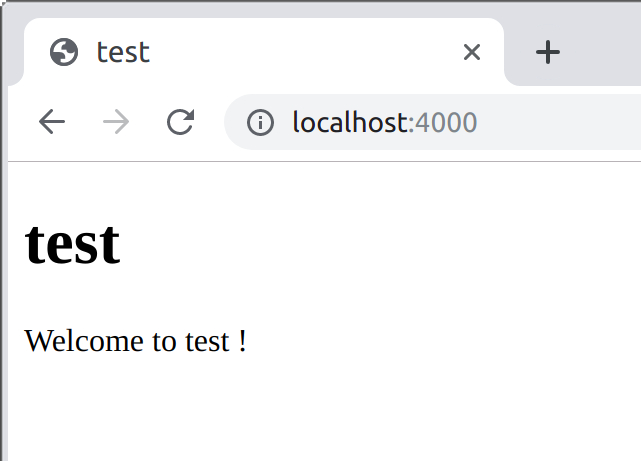
\includegraphics[width = 6cm]{test.jpg}
    \label{localhost:4000}
  \end{figure}
\end{frame}

\end{document}
